 \documentclass[a4paper,10pt]{article}
 \usepackage{tikz}
 \usepackage{fullpage}
 \usetikzlibrary{positioning,shadows,arrows,trees,shapes,fit}
 \begin{document}
 \begin{figure}
 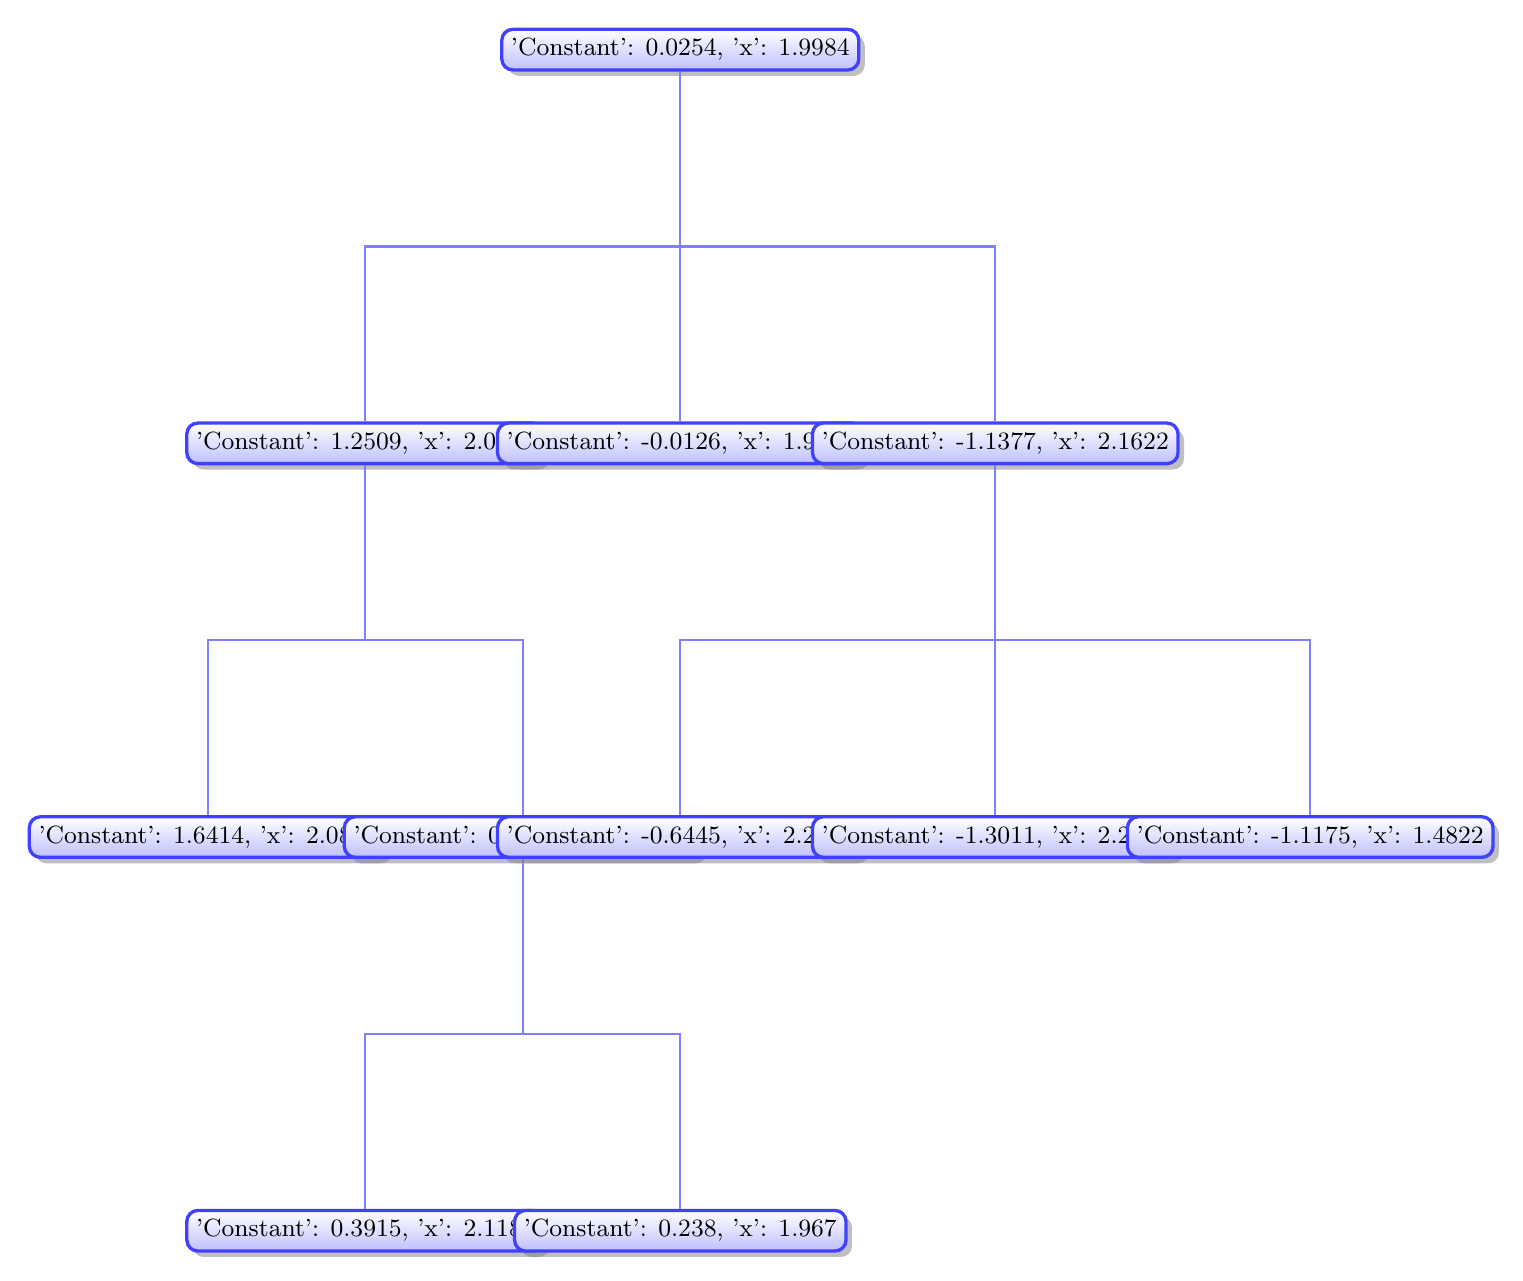
\begin{tikzpicture}
 [font=\small, edge from parent fork down, 
 every node/.style={top color=white, bottom color=blue!25, 
 	rectangle,rounded corners, minimum size=5mm, draw=blue!75,
	very thick, drop shadow, align=center},
 edge from parent/.style={draw=blue!50,thick},
 level 1/.style={sibling distance=4cm},
 level 2/.style={sibling distance=4cm}, 
 level 3/.style={sibling distance=4cm}, 
 level 4/.style={sibling distance=4cm}, 
 level 5/.style={sibling distance=4cm}, 
 level 6/.style={sibling distance=4cm}, 
 level distance=2cm,
 level distance=5cm,
 ]
\node {{'Constant': 0.0254, 'x': 1.9984}} %root
child { node {{'Constant': 1.2509, 'x': 2.0997}}  
child { node {{'Constant': 1.6414, 'x': 2.0863}}  
 }
child { node {{'Constant': 0.3478, 'x': 2.0822}}  
child { node {{'Constant': 0.3915, 'x': 2.1186}}  }
child { node {{'Constant': 0.238, 'x': 1.967}}  }
 }
 }
child { node {{'Constant': -0.0126, 'x': 1.9975}}  
 }
child { node {{'Constant': -1.1377, 'x': 2.1622}}  
child { node {{'Constant': -0.6445, 'x': 2.2275}}  
 }
child { node {{'Constant': -1.3011, 'x': 2.2082}}  
 }
child { node {{'Constant': -1.1175, 'x': 1.4822}}  
 }
 }
;\end{tikzpicture} 
 \caption{coefficient plot }  \end{figure}
\end{document} 
